\documentclass[paper=a4, fleqn]{scrartcl}
\usepackage[latin1]{inputenc}
\usepackage{dsfont}
\usepackage{color}
\usepackage{amsmath}
\usepackage{amssymb}
\usepackage{comment}
\usepackage{mathptmx}
\usepackage[scaled=.90]{helvet}
\usepackage{graphicx}
\usepackage{eucal}
\usepackage{palatino}
\usepackage{listings}
\usepackage{textcomp}


\begin{document}

\author{Faeze}

\begin{titlepage}

\begin{center}
Converting Polar Plot to PDF
\end{center}

\section{Parameters}

\subsection{Initial Values}

$alpha = 0.0
\newline
delta\_alpha = 0.0
\newline
delta\_trans = 0.0
\newline
plotrange\_min = 0.0
\newline
plotrange\_max = 1.0
\newline
frac\_noplot = 0.3
\newline
strech\_residual = 0.0
\newline
strech\_quasibrittle = 0.0
\newline
\newline$

\section{show Plot}

\subsection{Initial Plot, Function Polar plots and Unit Circle Plot}

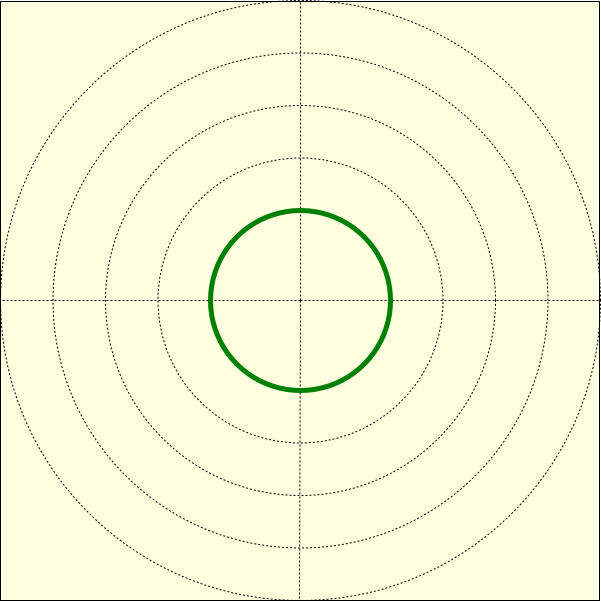
\includegraphics[scale=0.6]{polar_plot_initial.png}

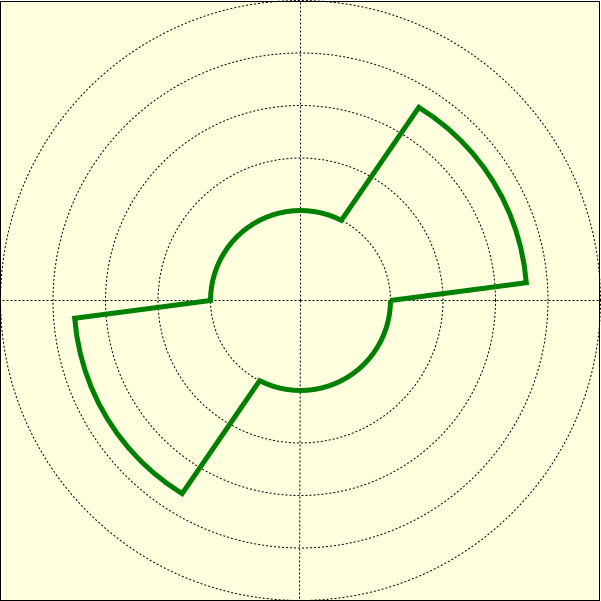
\includegraphics[scale=0.6]{polar_fn1_plot.png}

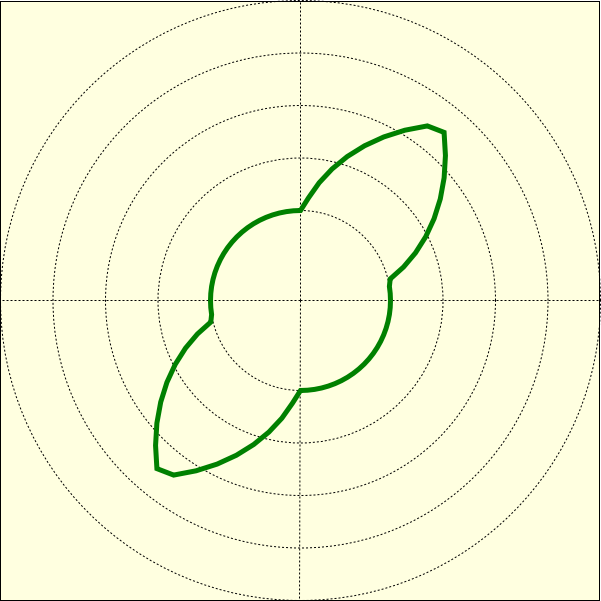
\includegraphics[scale=0.6]{polar_fn2_plot.png}

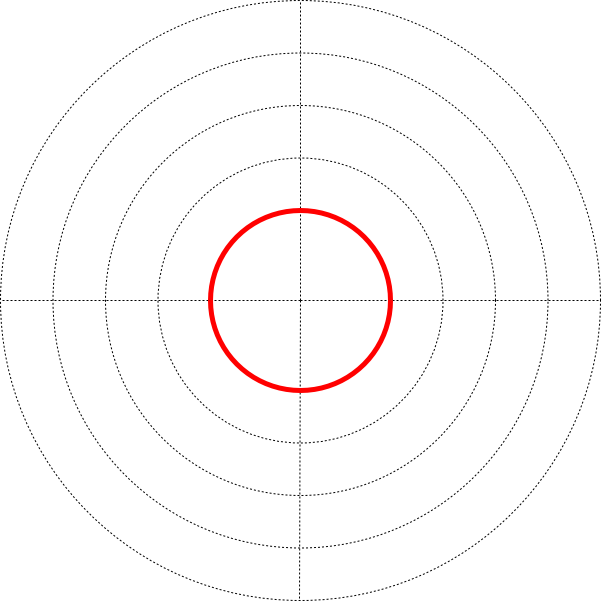
\includegraphics[scale=0.6]{polar_uc_plot.png}

\end{titlepage}

\end{document}
